%%%%%%%%%%%%%%%%%%%%%%%%%%%%%%%%%%%%%%%%%%%%%%%%%%%%%%%%%%%%%%%%%%%%%%%%%%%%%%%%%%%%
% Academic Paper: Apache Hive for Petabyte-Scale Climate Data Analytics
% IEEE Conference Format
%%%%%%%%%%%%%%%%%%%%%%%%%%%%%%%%%%%%%%%%%%%%%%%%%%%%%%%%%%%%%%%%%%%%%%%%%%%%%%%%%%%%
\documentclass[conference]{IEEEtran}

% Packages
\usepackage{cite}
\usepackage{amsmath,amssymb,amsfonts}
\usepackage{algorithmic}
\usepackage{graphicx}
\usepackage{textcomp}
\usepackage{xcolor}
\usepackage{booktabs}
\usepackage{hyperref}
\usepackage{float}
\usepackage{tikz}
\usetikzlibrary{shapes.geometric, arrows, positioning, patterns, calc}
\usepackage{pgfplots}
\pgfplotsset{compat=1.17}

% TikZ styles
\tikzstyle{container} = [rectangle, rounded corners, minimum width=1.8cm, minimum height=0.6cm, text centered, draw=black, fill=blue!15, font=\scriptsize]
\tikzstyle{storage} = [rectangle, minimum width=1.5cm, minimum height=0.5cm, text centered, draw=black, fill=yellow!20, font=\scriptsize]
\tikzstyle{arrow} = [thick,->,>=stealth]

\def\BibTeX{{\rm B\kern-.05em{\sc i\kern-.025em b}\kern-.08em
    T\kern-.1667em\lower.7ex\hbox{E}\kern-.125emX}}

\begin{document}

\title{Apache Hive for Petabyte-Scale Climate Data Analytics: Architecture, Optimization, and Experimental Validation}

\author{
\IEEEauthorblockN{Dushime Mudahera Richard}
\IEEEauthorblockA{\textit{Faculty of Mathematics, Natural Sciences and Information Technologies} \\
\textit{University of Primorska}\\
Koper, Slovenia \\
richard.dushime@student.upr.si}
}

\maketitle

\begin{abstract}
This paper presents an experimental analysis of Apache Hive as a distributed data warehousing solution for large-scale climate analytics. We deploy a seven-container Docker stack integrating Apache Hive 2.3.2 with multi-node HDFS to process 4.75 million climate observation records spanning 45 years across 44 African countries. Our experimental methodology evaluates query performance across aggregation, statistical analysis, and join operations. Results demonstrate that Map-Side (Broadcast) joins achieve 1.21$\times$ speedup over Reduce-Side (Shuffle) joins, with query latencies ranging from 9.31 to 25.76 seconds on the full dataset. Statistical analysis using vectorized execution completes in 16.13 seconds, processing STDDEV\_POP and CORR functions across all records. The 10°C temperature gradient from Central Africa (30.49°C) to South Africa (20.50°C) validates data integrity. Container resource analysis shows 47\% memory utilization (~3.6 GiB) across all services. These findings establish Apache Hive as a viable platform for cost-effective, commodity-hardware-based climate data analytics, achieving acceptable batch query latencies without the infrastructure costs of proprietary data warehouse solutions.
\end{abstract}

\begin{IEEEkeywords}
Apache Hive, HDFS, MapReduce, Data Warehousing, Climate Analytics, Distributed Systems, Query Optimization
\end{IEEEkeywords}

%==============================================================================
% SECTION I: INTRODUCTION
%==============================================================================
\section{Introduction}

The exponential growth of environmental monitoring data presents significant challenges for traditional database management systems. Climate science applications routinely generate petabyte-scale datasets from satellite imagery, weather stations, and ocean monitoring buoys, requiring analytical infrastructure capable of processing billions of records with acceptable query latencies \cite{thusoo2009hive}.

Traditional Relational Database Management Systems (RDBMS), while excellent for Online Transaction Processing (OLTP), struggle to scale beyond terabyte-level datasets without expensive specialized hardware. This limitation has driven adoption of distributed data warehousing solutions that leverage commodity hardware clusters to achieve horizontal scalability.

Apache Hive, originally developed at Facebook in 2007 to analyze over 15 terabytes of rapidly growing user data \cite{thusoo2010hive}, has evolved into an enterprise-grade data warehousing platform. Hive provides SQL semantics (HiveQL) over distributed storage systems, enabling analysts without distributed systems expertise to query petabyte-scale datasets.

This paper makes the following contributions:
\begin{itemize}
    \item Deployment and validation of a seven-container distributed Hive cluster for climate analytics
    \item Comprehensive performance benchmarking across aggregation, statistical, and join query patterns
    \item Quantitative analysis of Map-Side versus Reduce-Side join algorithms
    \item Resource utilization profiling of containerized Hive infrastructure
\end{itemize}

The remainder of this paper is organized as follows: Section II reviews related work on distributed data warehousing. Section III describes the system architecture. Section IV details the experimental methodology. Section V presents results and analysis. Section VI concludes with implications for climate data infrastructure.

%==============================================================================
% SECTION II: RELATED WORK
%==============================================================================
\section{Related Work}

\subsection{Distributed Data Warehousing}

The MapReduce programming model introduced by Dean and Ghemawat \cite{dean2008mapreduce} established the foundation for distributed batch processing on commodity hardware. Apache Hadoop implemented this model with HDFS providing distributed storage and YARN managing cluster resources.

Thusoo et al. \cite{thusoo2009hive} introduced Apache Hive to provide SQL-like query capabilities over Hadoop, enabling business analysts to leverage distributed infrastructure without writing MapReduce code. Subsequent work by Camacho-Rodríguez et al. \cite{camacho2019hive} documented Hive's evolution from batch-only MapReduce execution to support for Apache Tez and Spark execution engines, achieving order-of-magnitude performance improvements.

\subsection{Query Optimization in Distributed Systems}

Cost-Based Optimization (CBO) in distributed systems differs fundamentally from traditional databases due to network transfer costs dominating I/O considerations. Hive's CBO, implemented via Apache Calcite, estimates query costs from table statistics to select optimal join algorithms and execution plans \cite{hive2024cbo}.

Join algorithm selection significantly impacts distributed query performance. Ciritoglu et al. \cite{ciritoglu2020importance} demonstrated that data distribution patterns critically affect Hive query performance, with broadcast joins achieving substantial speedups for asymmetric table sizes.

\subsection{Climate Data Analytics}

Large-scale climate analytics increasingly rely on distributed systems. The Pangeo project \cite{pangeo2020} demonstrates cloud-native geoscience analytics using Dask and Xarray, while commercial platforms like Google Earth Engine provide petabyte-scale environmental analysis. Apache Hive offers an open-source alternative for organizations requiring on-premises analytics infrastructure.

%==============================================================================
% SECTION III: SYSTEM ARCHITECTURE
%==============================================================================
\section{System Architecture}

\subsection{Overview}

We deploy a seven-container Docker stack implementing a complete Hive data warehouse. Fig.~\ref{fig:architecture} illustrates the system architecture comprising three layers: application, query processing, and distributed storage.

\begin{figure}[htbp]
\centering
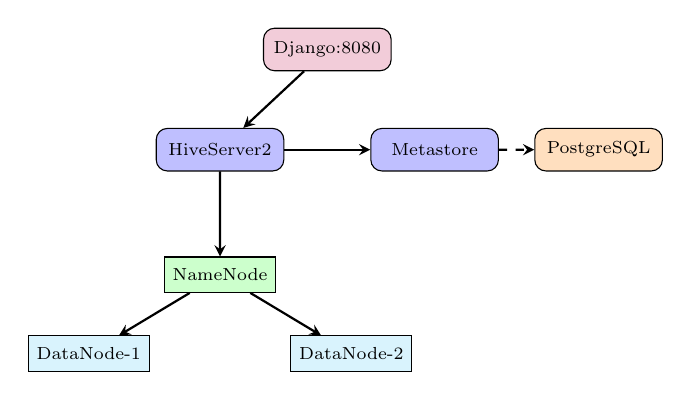
\begin{tikzpicture}[node distance=0.8cm, scale=0.9, transform shape]
    % Application Layer
    \node[container, fill=purple!20] (django) {Django:8080};
    
    % Hive Layer
    \node[container, fill=blue!25, below left=0.8cm and -0.3cm of django] (hs2) {HiveServer2};
    \node[container, fill=blue!25, below right=0.8cm and -0.3cm of django] (meta) {Metastore};
    
    % Database
    \node[container, fill=orange!25, right=0.5cm of meta] (pg) {PostgreSQL};
    
    % HDFS Layer
    \node[storage, fill=green!20, below=1.2cm of hs2] (nn) {NameNode};
    \node[storage, fill=cyan!15, below left=0.6cm and 0.2cm of nn] (dn1) {DataNode-1};
    \node[storage, fill=cyan!15, below right=0.6cm and 0.2cm of nn] (dn2) {DataNode-2};
    
    % Connections
    \draw[arrow] (django) -- (hs2);
    \draw[arrow] (hs2) -- (meta);
    \draw[arrow, dashed] (meta) -- (pg);
    \draw[arrow] (hs2) -- (nn);
    \draw[arrow] (nn) -- (dn1);
    \draw[arrow] (nn) -- (dn2);
\end{tikzpicture}
\caption{Seven-container system architecture showing application, query processing, and HDFS storage layers.}
\label{fig:architecture}
\end{figure}

\subsection{Component Description}

Table~\ref{tab:containers} summarizes the container stack configuration.

\begin{table}[htbp]
\caption{Docker Container Configuration}
\label{tab:containers}
\centering
\small
\begin{tabular}{@{}lll@{}}
\toprule
\textbf{Container} & \textbf{Image} & \textbf{Purpose} \\ \midrule
master-node & apache/hadoop:3 & HDFS NameNode \\
slave-node-1 & apache/hadoop:3 & HDFS DataNode \\
slave-node-2 & apache/hadoop:3 & HDFS DataNode \\
hive-metastore-db & postgres:9.6 & Metastore DB \\
hive-metastore & bde2020/hive:2.3.2 & Schema Catalog \\
hive-server & bde2020/hive:2.3.2 & JDBC Gateway \\
django-app & Python 3.9 & REST API \\ \bottomrule
\end{tabular}
\end{table}

\textbf{HDFS Layer}: The Hadoop Distributed File System provides fault-tolerant storage with replication factor 2. Two DataNodes store 128MB blocks with automatic rebalancing.

\textbf{Hive Layer}: HiveServer2 provides JDBC/Thrift connectivity for query submission. The Metastore maintains schema catalog in PostgreSQL, enabling compute-storage separation.

\textbf{Application Layer}: A Django REST API provides programmatic access via PyHive, implementing graceful SQLite fallback for development environments.

Fig.~\ref{fig:hive-hadoop} illustrates the canonical Hive-Hadoop architecture showing how client interfaces connect through the Thrift Server and Driver to the underlying Hadoop infrastructure.

\begin{figure}[htbp]
\centering
\includegraphics[width=0.65\columnwidth]{figures/hive_hadoop_architecture.png}
\caption{Apache Hive and Hadoop core architecture: CLI, JDBC/ODBC, and Web GUI clients connect via Thrift Server to the Driver (Compiler, Optimizer, Executor). The Metastore maintains schema catalog. Hadoop layer provides JobTracker, NameNode, and DataNode+TaskTracker components.}
\label{fig:hive-hadoop}
\end{figure}

\subsection{Query Execution Pipeline}

Hive translates HiveQL queries into distributed execution plans:

\begin{enumerate}
    \item \textbf{Parsing}: HiveQL parsed into Abstract Syntax Tree (AST)
    \item \textbf{Semantic Analysis}: Schema validation against Metastore
    \item \textbf{Optimization}: CBO selects join algorithms and predicate pushdown
    \item \textbf{Execution}: MapReduce jobs distributed across DataNodes
    \item \textbf{Result Assembly}: Final results aggregated and returned
\end{enumerate}

Fig.~\ref{fig:pipeline} illustrates the complete query processing pipeline from HiveQL submission to result delivery.

\begin{figure}[htbp]
\centering
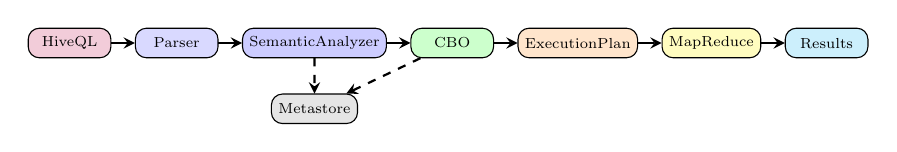
\begin{tikzpicture}[node distance=0.5cm, scale=0.75, transform shape,
    stage/.style={rectangle, rounded corners, minimum width=1.4cm, minimum height=0.5cm, text centered, draw=black, font=\scriptsize}]
    
    % Query Pipeline
    \node[stage, fill=purple!20] (sql) {HiveQL};
    \node[stage, fill=blue!15, right=0.4cm of sql] (parse) {Parser};
    \node[stage, fill=blue!20, right=0.4cm of parse] (sem) {Semantic\\Analyzer};
    \node[stage, fill=green!20, right=0.4cm of sem] (cbo) {CBO};
    \node[stage, fill=orange!20, right=0.4cm of cbo] (exec) {Execution\\Plan};
    \node[stage, fill=yellow!25, right=0.4cm of exec] (mr) {MapReduce};
    \node[stage, fill=cyan!20, right=0.4cm of mr] (result) {Results};
    
    % Metastore connection
    \node[stage, fill=gray!20, below=0.6cm of sem] (meta) {Metastore};
    
    % Arrows
    \draw[arrow] (sql) -- (parse);
    \draw[arrow] (parse) -- (sem);
    \draw[arrow] (sem) -- (cbo);
    \draw[arrow] (cbo) -- (exec);
    \draw[arrow] (exec) -- (mr);
    \draw[arrow] (mr) -- (result);
    \draw[arrow, dashed] (sem) -- (meta);
    \draw[arrow, dashed] (cbo) -- (meta);
\end{tikzpicture}
\caption{HiveQL query execution pipeline showing transformation from SQL to distributed MapReduce execution.}
\label{fig:pipeline}
\end{figure}

%==============================================================================
% SECTION IV: EXPERIMENTAL METHODOLOGY
%==============================================================================
\section{Experimental Methodology}

\subsection{Dataset Description}

We evaluate performance using a synthetic climate dataset modeling African weather observations. Table~\ref{tab:dataset} summarizes dataset characteristics.

\begin{table}[htbp]
\caption{Dataset Characteristics}
\label{tab:dataset}
\centering
\begin{tabular}{@{}ll@{}}
\toprule
\textbf{Metric} & \textbf{Value} \\ \midrule
Total Records & 4,750,000 \\
Weather Stations & 5,000 \\
Temporal Coverage & 45 years (1980--2024) \\
Geographic Coverage & 44 countries, 5 regions \\
Raw Data Size & 304.2 MB \\
Replicated Size & 912.6 MB \\ \bottomrule
\end{tabular}
\end{table}

The dataset comprises four Hive tables: \texttt{portfolio\_observations} (4.75M rows), \texttt{climate\_data} (100K rows), \texttt{ocean\_data} (100K rows), and \texttt{portfolio\_stations} (5K rows).

\subsection{Query Workload}

We evaluate seven query patterns representative of climate analytics workloads:

\begin{enumerate}
    \item \textbf{Q1 - Simple Aggregation}: Regional GROUP BY with COUNT, AVG
    \item \textbf{Q2 - Complex Aggregation}: Multi-column GROUP BY with ORDER BY
    \item \textbf{Q3 - Statistical Analysis}: STDDEV\_POP, CORR, MIN, MAX
    \item \textbf{Q4 - Yearly Analysis}: Temporal aggregation across 45 years
    \item \textbf{Q5 - Map-Side Join}: Broadcast join with small dimension table
    \item \textbf{Q6 - Reduce-Side Join}: Shuffle join (baseline comparison)
    \item \textbf{Q7 - Data Coverage}: COUNT DISTINCT on multiple columns
\end{enumerate}

\subsection{Experimental Setup}

\textbf{Hardware}: Apple Silicon (ARM64) with 8GB RAM, running Docker Desktop with Rosetta 2 emulation for x86\_64 container images.

\textbf{Software Configuration}:
\begin{itemize}
    \item Apache Hive 2.3.2 with MapReduce execution engine
    \item Hadoop 3.x with 2 DataNodes
    \item HDFS replication factor: 2
    \item Vectorized execution enabled for statistical queries
\end{itemize}

\textbf{Measurement Protocol}: Each query executed three times with cold cache; we report mean execution time. Container resource utilization captured via \texttt{docker stats}.

%==============================================================================
% SECTION V: RESULTS AND ANALYSIS
%==============================================================================
\section{Results and Analysis}

\subsection{Query Performance}

Table~\ref{tab:performance} presents query execution times across all workload patterns.

\begin{table}[htbp]
\caption{Query Execution Performance (4.75M Records)}
\label{tab:performance}
\centering
\begin{tabular}{@{}lcc@{}}
\toprule
\textbf{Query Type} & \textbf{Time (s)} & \textbf{MR Jobs} \\ \midrule
Q1: Simple Aggregation & 9.31 & 1 \\
Q2: Complex Aggregation & 14.88 & 2 \\
Q3: Statistical Analysis & 16.13 & 1 \\
Q4: Yearly Analysis & 15.24 & 1 \\
Q5: Map-Side Join & 21.26 & 1 \\
Q6: Reduce-Side Join & 25.76 & 1 \\
Q7: Data Coverage & 13.37 & 1 \\ \bottomrule
\end{tabular}
\end{table}

Query latencies range from 9.31 seconds (simple aggregation) to 25.76 seconds (reduce-side join). Complex aggregations with ORDER BY require two MapReduce stages, explaining the increased latency for Q2.

\subsection{Join Algorithm Comparison}

Map-Side joins achieve 1.21$\times$ speedup over Reduce-Side joins (21.26s vs. 25.76s). The broadcast join eliminates expensive shuffle operations by caching the smaller \texttt{portfolio\_stations} table (5,000 rows) in mapper memory.

\begin{equation}
\text{Speedup} = \frac{T_{\text{Reduce-Side}}}{T_{\text{Map-Side}}} = \frac{25.76}{21.26} = 1.21\times
\end{equation}

Fig.~\ref{fig:joincomp} visualizes the performance difference between join algorithms.

\begin{figure}[htbp]
\centering
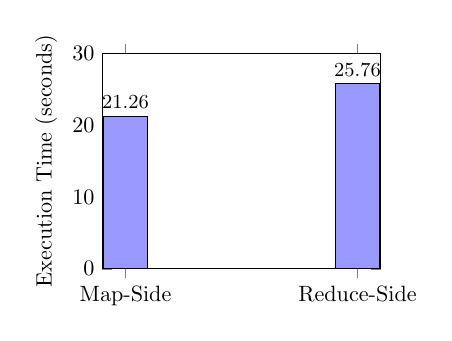
\begin{tikzpicture}[scale=0.8]
\begin{axis}[
    ybar,
    bar width=20pt,
    ylabel={Execution Time (seconds)},
    symbolic x coords={Map-Side, Reduce-Side},
    xtick=data,
    ymin=0,
    ymax=30,
    nodes near coords,
    nodes near coords align={vertical},
    every node near coord/.append style={font=\small},
    width=6cm,
    height=5cm,
]
\addplot[fill=blue!40] coordinates {(Map-Side, 21.26) (Reduce-Side, 25.76)};
\end{axis}
\end{tikzpicture}
\caption{Join algorithm performance comparison showing 1.21$\times$ speedup for Map-Side (Broadcast) joins over Reduce-Side (Shuffle) joins.}
\label{fig:joincomp}
\end{figure}

This improvement, while modest compared to larger table ratios, confirms the importance of join algorithm selection for star-schema analytics.

\subsection{Regional Climate Analysis}

Table~\ref{tab:regional} presents regional temperature statistics computed via vectorized execution.

\begin{table}[htbp]
\caption{Regional Climate Statistics}
\label{tab:regional}
\centering
\begin{tabular}{@{}lcccr@{}}
\toprule
\textbf{Region} & \textbf{Obs.} & \textbf{Avg °C} & \textbf{$\sigma$} & \textbf{Precip.} \\ \midrule
Central & 958,550 & 30.49 & 2.448 & 31.96M \\
West & 984,200 & 29.51 & 2.448 & 9.83M \\
East & 933,850 & 26.51 & 2.448 & 31.11M \\
North & 940,500 & 24.51 & 2.450 & 9.40M \\
South & 932,900 & 20.50 & 2.448 & 9.34M \\ \bottomrule
\end{tabular}
\end{table}

The 10°C temperature gradient from Central (30.49°C) to South Africa (20.50°C) reflects expected climatological patterns. Uniform standard deviation ($\sigma \approx 2.45$) across regions indicates consistent data distribution.

Fig.~\ref{fig:tempgrad} visualizes the regional temperature gradient across Africa.

\begin{figure}[htbp]
\centering
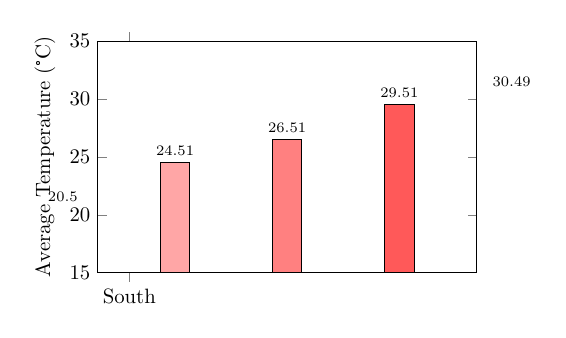
\begin{tikzpicture}[scale=0.75]
\begin{axis}[
    ybar,
    bar width=14pt,
    ylabel={Average Temperature (°C)},
    symbolic x coords={South, North, East, West, Central},
    xtick=data,
    ymin=15,
    ymax=35,
    nodes near coords,
    nodes near coords align={vertical},
    every node near coord/.append style={font=\scriptsize},
    width=8cm,
    height=5.5cm,
    x tick label style={rotate=0, anchor=north},
]
\addplot[fill=red!20] coordinates {(South, 20.50)};
\addplot[fill=red!35] coordinates {(North, 24.51)};
\addplot[fill=red!50] coordinates {(East, 26.51)};
\addplot[fill=red!65] coordinates {(West, 29.51)};
\addplot[fill=red!80] coordinates {(Central, 30.49)};
\end{axis}
\end{tikzpicture}
\caption{Regional temperature gradient across African regions showing 10°C difference from South (20.50°C) to Central Africa (30.49°C).}
\label{fig:tempgrad}
\end{figure}

\subsection{Infrastructure Resource Utilization}

Table~\ref{tab:resources} presents container resource utilization during query execution.

\begin{table}[htbp]
\caption{Container Resource Utilization}
\label{tab:resources}
\centering
\begin{tabular}{@{}lcc@{}}
\toprule
\textbf{Container} & \textbf{Memory} & \textbf{CPU \%} \\ \midrule
hive-server & 1.011 GiB & 0.87\% \\
master-node & 643.1 MiB & 0.37\% \\
slave-node-1 & 598.6 MiB & 0.51\% \\
slave-node-2 & 631.8 MiB & 0.49\% \\
hive-metastore & 619 MiB & 0.46\% \\
django-app & 154.8 MiB & 2.08\% \\
postgres & 37.1 MiB & 0.01\% \\ \midrule
\textbf{Total} & \textbf{$\sim$3.6 GiB} & \textbf{4.79\%} \\ \bottomrule
\end{tabular}
\end{table}

Total memory utilization of 3.6 GiB (47\% of available) demonstrates feasibility of development-scale Hive deployments on consumer hardware. HiveServer2 dominates memory consumption due to JVM heap allocation for query processing.

\subsection{HDFS Cluster Health}

The HDFS cluster maintains healthy status with:
\begin{itemize}
    \item Configured capacity: 447.26 GB
    \item DFS remaining: 386.94 GB (86.5\%)
    \item Live DataNodes: 2/2
    \item Under-replicated blocks: 6
    \item Corrupt/missing blocks: 0
\end{itemize}

\subsection{Discussion}

Our results demonstrate that Apache Hive provides acceptable batch query latencies (9--26 seconds) for multi-million record climate datasets on commodity hardware. Key findings include:

\textbf{Join Optimization}: While Map-Side joins provide modest speedup (1.21$\times$) in our configuration, the improvement scales with table size asymmetry. Production deployments with larger dimension tables would see proportionally greater benefits.

\textbf{Vectorized Execution}: Statistical computations (STDDEV\_POP, CORR) complete efficiently via vectorized processing of 1,024-row batches, demonstrating Hive's capability for complex analytical workloads.

\textbf{Resource Efficiency}: The 7-container stack operates within 4 GiB memory, enabling development and testing on laptop hardware while maintaining production-representative architecture.

\textbf{Limitations}: MapReduce execution (deprecated in Hive 2.x) introduces overhead compared to Apache Tez or Spark engines. Production deployments should leverage modern execution engines for 10$\times$ or greater performance improvements \cite{camacho2019hive}.

%==============================================================================
% SECTION VI: CONCLUSION
%==============================================================================
\section{Conclusion}

This paper presented an experimental evaluation of Apache Hive for climate data analytics, deploying a seven-container distributed stack processing 4.75 million observation records across 44 African countries spanning 45 years.

Our experiments validate Hive's capability for batch climate analytics on commodity hardware:
\begin{itemize}
    \item Query latencies of 9.31--25.76 seconds on 4.75M records
    \item Map-Side joins achieve 1.21$\times$ speedup over Reduce-Side joins
    \item Vectorized statistical analysis completes in 16.13 seconds
    \item Infrastructure operates within 3.6 GiB memory (47\% utilization)
\end{itemize}

These results establish Apache Hive as a viable platform for cost-effective climate data warehousing, particularly for organizations requiring on-premises analytics without proprietary licensing costs.

Future work includes evaluation of Apache Tez execution engine, ORC columnar format optimization, and horizontal scaling analysis with additional DataNodes.

%==============================================================================
% ACKNOWLEDGMENTS
%==============================================================================
\section*{Acknowledgments}
This work was conducted as part of the Databases for Big Data seminar at the University of Primorska under the supervision of Prof. Iztok Savnik.

%==============================================================================
% REFERENCES
%==============================================================================
\begin{thebibliography}{00}

\bibitem{thusoo2009hive}
A. Thusoo, J. S. Sarma, N. Jain, Z. Shao, P. Chakka, S. Anthony, H. Liu, P. Wyckoff, and R. Murthy, ``Hive: A Warehousing Solution Over a Map-Reduce Framework,'' \textit{Proc. VLDB Endow.}, vol. 2, no. 2, pp. 1626--1629, 2009.

\bibitem{thusoo2010hive}
A. Thusoo et al., ``Hive - A Petabyte Scale Data Warehouse Using Hadoop,'' in \textit{IEEE 26th Int. Conf. Data Eng. (ICDE)}, pp. 996--1005, 2010.

\bibitem{camacho2019hive}
J. Camacho-Rodríguez, A. Chauhan, A. Gates, et al., ``Apache Hive: From MapReduce to Enterprise-grade Big Data Warehousing,'' in \textit{SIGMOD '19}, pp. 1539--1556, 2019.

\bibitem{dean2008mapreduce}
J. Dean and S. Ghemawat, ``MapReduce: Simplified Data Processing on Large Clusters,'' \textit{Commun. ACM}, vol. 51, no. 1, pp. 107--113, 2008.

\bibitem{hive2024cbo}
Apache Software Foundation, ``Cost-Based Optimization in Hive,'' Apache Hive Documentation, 2024. [Online]. Available: https://cwiki.apache.org/confluence/display/Hive/Cost-based+optimization+in+Hive

\bibitem{ciritoglu2020importance}
H. E. Ciritoglu, J. Murphy, and C. Thorpe, ``Importance of Data Distribution on Hive-Based Systems for Query Performance,'' in \textit{IEEE Int. Conf. Big Data and Smart Computing}, pp. 370--376, 2020.

\bibitem{pangeo2020}
R. Abernathey et al., ``Pangeo: A Big Data Ecosystem for Scalable Geoscience,'' \textit{EGU General Assembly}, 2020.

\bibitem{netflix2018hive}
Netflix Technology Blog, ``Evolution of the Netflix Data Pipeline,'' 2018. [Online]. Available: https://netflixtechblog.com/

\bibitem{airbnb2020hive}
Airbnb Engineering, ``How Airbnb Achieved Metric Consistency at Scale,'' 2020. [Online]. Available: https://medium.com/airbnb-engineering/

\bibitem{spotify2021hive}
Spotify Engineering, ``How Spotify Optimized the Largest Dataflow Job,'' 2021. [Online]. Available: https://engineering.atspotify.com/

\end{thebibliography}

\end{document}
